\documentclass[crop=false,fleqn]{standalone}
\usepackage{../../../globle-preamble}

\begin{document}
    \textbf{Express the perimeter $P$ of square as a function of its area $A$.}

    \begin{center}
        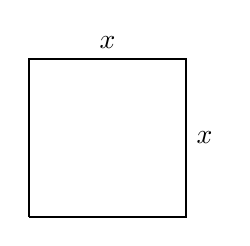
\begin{tikzpicture}
            \draw[thick] (0,0) --  (0,2) -- node[above]{$x$} (2,2)
                -- node[right]{$x$} (2,0) -- (0,0);
        \end{tikzpicture}
    \end{center}

    Let,

    \begin{equation*}
        \begin{split}
            \text{Length of square} = L &= x \\
            \text{Width of square} = W &= x \\
            \\
            \text{Perimeter of square} = P &= 2(L+W) \\
                                        &= 2(x+x) \\
                                        &= 4x \\
            \\
            \text{Area of square} = A &= L \times W \\
                                    &= x \times x \\
                                    &= x^2 \\
                        \implies x &= \sqrt{A}
        \end{split}
    \end{equation*}

    As $P=4x$ and $x=\sqrt{4}$ we can derive that

    \begin{equation*}
        P=4\sqrt{A}
    \end{equation*}

    The above relation expresses the perimeter $P$ of a sqaure as its area $A$.
\end{document}
